\documentclass[aspectratio=169,xcolor=dvipsnames]{beamer}

\usepackage{hyperref}
\usepackage{graphicx}
\usepackage{booktabs}
\usepackage{amsmath}
\usepackage{lipsum}
\usepackage{natbib}

\hypersetup{
	colorlinks=true,
	linkcolor=blue,
	filecolor=magenta,
	urlcolor=blue,
	citecolor=blue,
	pdfpagemode=FullScreen,
}

% Tema do beammer. Para mais opções acesse:
% https://www.overleaf.com/learn/latex/Beamer
\usetheme{Madrid}
\usecolortheme{whale}

% Pacotes para fontes
\RequirePackage[T1]{fontenc}
\RequirePackage[brazil]{babel}
\RequirePackage[utf8]{inputenc}

% Justificando o texto
\usepackage{ragged2e}
\usepackage{etoolbox}
\apptocmd{\frame}{}{\justifying}{}
\renewcommand{\raggedright}{\leftskip=0pt \rightskip=0pt plus 0cm}

% Configuração do espaçamento dos parágrafos
\usepackage{parskip}
\setlength{\parskip}{0.5\baselineskip plus 0.5pt minus 0.5pt} 

% Destaque de cores
\usepackage{xcolor, soul}
\newcommand\destaque[2]{\textcolor{#2}{\textbf{#1}}} %minúsculo
\newcommand\Destaque[2]{\textcolor{#2}{\uppercase{\textbf{#1}}}} % maiúsculo
\newcommand\realce[1]{\colorbox{yellow}{#1}} % maiúsculo

% Inclusão de logo
\logo{
\includegraphics[height=0.5cm]{uninove-logo}}

% Remove os símbolos de navegação no rodapé
\setbeamertemplate{navigation symbols}{}

% Configure os parâmetros abaixo de acordo com a sua necessidade
\title[\color{white}{Título no Rodapé}]{Disciplina}
\subtitle{Subtítulo}
\author[Nome do Autor]{Nome do Autor}
\institute[Universidade Nove de Julho]{Universidade Nove de Julho}
\date{\today}

% Cabeçalho do documento
\begin{document}

\begin{frame}
    \titlepage
\end{frame}

\begin{frame}{Sumário}
    \tableofcontents
\end{frame}

% Slide de título
\section{Parágrafos Simples}
\begin{frame}
    \center \Huge Parágrafos
\end{frame}

% Página de slide
\begin{frame}{Título}{Subtítulo}
    Olá, \Destaque{Bom dia}{red}. Esse é um \destaque{parágrafo}{blue} com partes em ``destaque''. Tem um formato diferente do \destaque{\textit{boxcolor}}{green}.

    Realce de palavras \realce{\destaque{parágrafo}{black}}.    

    \lipsum[4]

    \lipsum[2-2][2-5]

\end{frame}

% Slide de título
\begin{frame}
    \center \Huge Listas
\end{frame}

% Página de slide
\begin{frame}{Lista simples}
    \begin{itemize}
        \item Primeiro;
        \item Segundo;
        \item Terceiro.
    \end{itemize}
\end{frame}

% Apresentado tópicos por nível
% Se aplica também ao "enumerate" a seguir
\begin{frame}{Lista numerada}
    \begin{enumerate}
        \item Primeiro;
        \item Segundo;
        \item Terceiro.
    \end{enumerate}
\end{frame}

\begin{frame}{Lista com nível (surgimento)}
    Ao abrir o \textit{slide}, o primeiro nível é apresentado. Os demais, a partir do clique, barra etc.
    \begin{enumerate}
        \item<1-> Primeiro;
        \item<2-> Segundo;
        \item<3-> Terceiro.
    \end{enumerate}
\end{frame}

% Destacando textos em blocos
\section{Destaque de texto em blocos}
\begin{frame}
    \center \Huge Destacando textos em blocos
\end{frame}
\begin{frame}{Azul, verde e vermelho}
    \begin{block}{Destaque azul}
        \lipsum[1][3-5]
    \end{block}

    \begin{exampleblock}{Destaque em verde}
        \lipsum[1][1-3]
    \end{exampleblock}

    \begin{alertblock}{Destaque em vermelho}
        \lipsum[1][5-7]
    \end{alertblock}
\end{frame}

% Slide de título
\section{Imagens}
\begin{frame}
    \center \Huge Incluindo imagens
\end{frame}

% Imagens
% Mais informações sobre imagens, acesse:
% https://www.overleaf.com/learn/latex/Inserting_Images
\begin{frame}{Uma imagem}
    \begin{figure}
        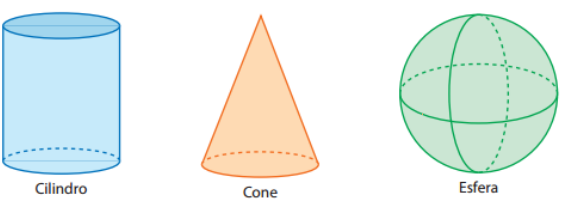
\includegraphics[width=0.8\linewidth]{img/imagem.png}
    \end{figure}
\end{frame}

% Configurar o tamanho para adequar à tela
\begin{frame}{Duas imagens}
    \begin{figure}
        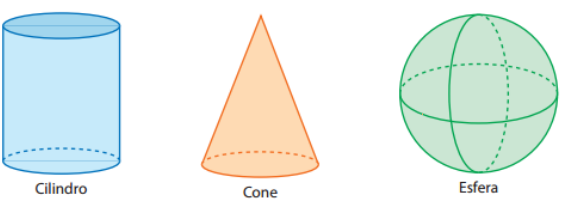
\includegraphics[width=0.5\linewidth]{img/imagem.png}
        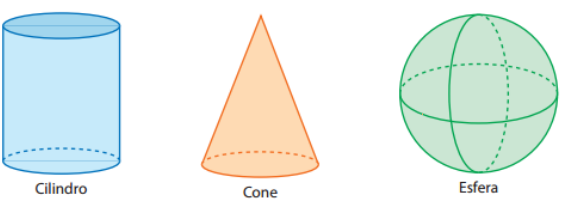
\includegraphics[width=0.5\linewidth]{img/imagem.png}
    \end{figure}
\end{frame}

% Configurar o tamanho para adequar à tela
\begin{frame}{Três ou mais imagens}
    \begin{figure}
        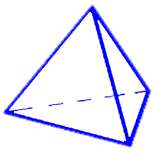
\includegraphics[width=0.2\linewidth]{img/img_01.png} \hspace{1cm}
        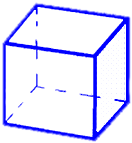
\includegraphics[width=0.2\linewidth]{img/img_02.png} \hspace{1cm}
        
\includegraphics[width=0.2\linewidth]{img/img_03.png}
    \end{figure}
    Citação indireta: A vida é bela \citep{p1}.

    Citação direta: Segundo \citet{p1}, "[...]a vida é bela".
    Citação direta: Segundo \citet{p2}, "[...]a vida é bela".
    Citação direta: Segundo \citet{p3}, "[...]a vida é bela".
\end{frame}

% Colunas
\begin{frame}{Colunas}
    \begin{columns}

        \begin{column}{0.48\textwidth}
            \lipsum[2-2]
        \end{column}
        
        % Coloca uma linha vertical entre as colunas
        \hspace{-10pt}
        \vrule{}

        \begin{column}{0.48\textwidth}
            \lipsum[2-2]
        \end{column}

    \end{columns}
\end{frame}

% Slide de títulos
\section{Referências}
\begin{frame}{Referências}
    
    \footnotesize{
        \thispagestyle{empty}
        \clearpage
        \begin{thebibliography}{5}
            % Um autor
            \bibitem[Sobrenome, 2021]{p1} \textbf{Sobrenome}, Nome.
            \newblock \textbf{Título da publicação}.
            \newblock \emph{Periódico} 12(3), 45 -- 678, 2021.
            \newblock DOI: \href{https://dx.doi.org/10.18607/ES201877599}{10.18607/ES201877599}

            % Dois autores
            \bibitem[Sobrenome1 e Sobrenome2, 2021]{p2} \textbf{Sobrenome1}, Nome1; \textbf{Sobrenome2}, Nome2.
            \newblock \textbf{Título da publicação}.
            \newblock \emph{Periódico} 12(3), 45 -- 678, 2021.
            \newblock DOI: \href{https://dx.doi.org/10.18607/ES201877599}{10.18607/ES201877599}

            % Três ou mais
            \bibitem[Sobrenome \textit{et al.}, 2021]{p3} \textbf{Sobrenome}, Nome \textit{et al.}
            \newblock \textbf{Título da publicação}.
            \newblock \emph{Periódico} 12(3), 45 -- 678, 2021.
            \newblock DOI: \href{https://dx.doi.org/10.18607/ES201877599}{10.18607/ES201877599}

        \end{thebibliography}
    }
\end{frame}

\begin{frame}
    \Huge{\centerline{\textbf{Até a próxima aula}}}
\end{frame}

\end{document}